\section{Conclusions}

\begin{figure}[htb!]
\centering
\tikzstyle{label}=[rectangle,rounded corners,minimum width=3cm,minimum height=1cm,text centered,draw=black,fill=gray!20]
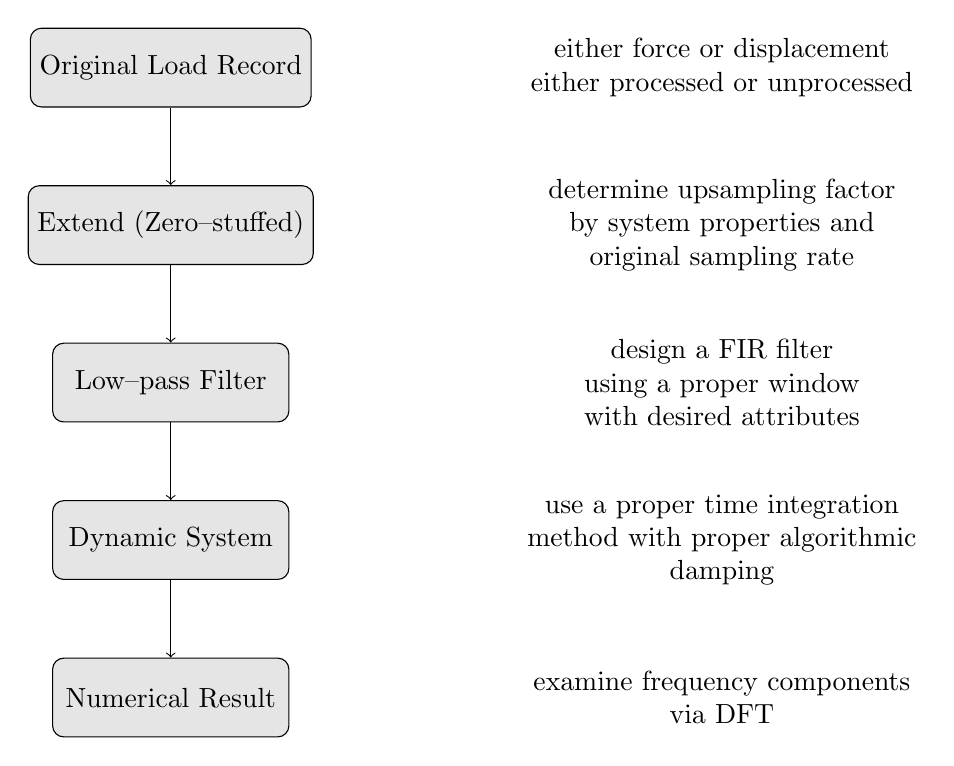
\begin{tikzpicture}
\node(original)[label]{Original Load Record};
\node(extended)[label,below of=original,yshift=-1cm]{Extend (Zero--stuffed)};
\node(filter)[label,below of=extended,yshift=-1cm]{Low--pass Filter};
\node(oscillator)[label,below of=filter,yshift=-1cm]{Dynamic System};
\node(system)[label,below of=oscillator,yshift=-1cm]{Numerical Result};
\draw[->](original)--(extended);
\draw[->](extended)--(filter);
\draw[->](filter)--(oscillator);
\draw[->](oscillator)--(system);
\node[xshift=6cm,right of=original,align=center]{either force or displacement\\either processed or unprocessed};
\node[xshift=6cm,right of=extended,align=center]{determine upsampling factor\\by system properties and\\original sampling rate};
\node[xshift=6cm,right of=filter,align=center]{design a FIR filter\\using a proper window\\with desired attributes};
\node[xshift=6cm,right of=oscillator,align=center]{use a proper time integration\\method with proper algorithmic\\damping};
\node[xshift=6cm,right of=system,align=center]{examine frequency components\\via DFT};
\end{tikzpicture}
\caption{typical analysis flow with recommendations}
\end{figure}

It is evident that the linear interpolation is not ideal.
\begin{enumerate}
\item In order to avoid linear interpolation, it is better to have the identical time step size and sampling interval. To this end, one shall first choose a proper time step size that would be used in numerical analysis, typically it is smaller than sampling interval. Then, the seismogram shall be upsampled.
\item The low--pass filter shall possess sufficiently small side lobe level.
\item Whether the time integration method possesses algorithmic damping does not affect the type of spurious damping force discussed in this work. The high frequency noise exists intrinsically and is spotted analytically. Algorithmic damping does not alleviate the issue in this regard.
\item The Rayleigh damping model undoubtedly introduces high damping forces in high frequencies. However, with sufficiently small, if not in absence of, high frequency components, the Rayleigh damping model can still be used. The spurious damping force can be suppressed.
\item It is still preferred to use an alternative damping model that does not produce unbounded damping action in regions out of interests.
\end{enumerate}

\begin{enumerate}
\item Determine whether the seismograph, in the form of either displacement or acceleration, is properly processed. Typical seismographs are preprocessed by applying a band--pass filter with bounds at around \SI{0.05}{\hertz} and \SIrange{25}{50}{\hertz} for structural analysis.
\item Determine a proper time step size and the corresponding upsampling ratio.
\item Design a proper upsampling filter so that time step size matches upsampling interval.
\item Avoid high frequency modes in the target structure. For example, use a properly integrated consistent mass matrix or full ranked diagonal mass matrix, limit the penalty factor within a reasonable range when it comes to model, for example, axial inextensibility. Constraints are better implemented via the Lagrange multiplier method.
\end{enumerate}

The numerical examples are carried out using \texttt{suanPan} \citep{Chang2022}. Scripts to generate figures and models can be found online.